\chap{Discussion and Evaluations}

The present study investigates about the possibility of testing the Data Science process using Python, trying to apply it to the Norwegian salmon farming industry, in order to gather and let be available as many useful results as possible about.\\
JUSTIFY YOUR APPROACH\\
Is possible to say that the results obtained are providing an answer to most of the initial objectives of this thesis. \\
In particular, this study shows that is actually possible to have a first approach to the Data Science field using Python and all the considerations reported during each step of the implementation are showing an overview of the Data Science process.\\
Further more, all the output results, such as graphic or coefficients value, are showing which kind of modules and packages Python provides in order to solve data analysis problems that allow to understand better Python potential in this field.\\
Since the implemented system is has a high reusability and high automatization level, is possible to use it in order to make the same initial data analysis, displayig and forecast in a really short time about different datasets composed by data coming from every kind of area of interest.\\
The results about the Norwegian salmon farming are actually not reporting any kind of new interesting informations. That because this thesis has been based mainly on the Data Science process and Python using more than a concrete information extraction.\\
Some useful results are anyway provided, such as a structured dataset, more accessable and readable, together with descriptions of the data that could be helpful in the future for more specific analysis in this area. Further more, is possible to check out clear and readable graphics about several parametrs of each single county of Norway that could be used for an initial view analysis. Also coefficients values are already calculated, and an initial forecast system allows to have a general idea about the future expectations in this area.


\newpage

\section{Evaluation System implemented}
The following results table allows to make several observations about it: \\
1) how is possible to see, the evaluation system provide ARIMA configuration that, tested with real future values, are providing a much higher MAPE value. \\
2) The only MAPE value that is almost the same of the one calculated during the evaluation sstem is the one about the Norway dataset. Would be useful to understand why.

 \begin{table}[ht]
\makebox[1\textwidth][c]{
    \begin{tabular}{ | l | l | l | l | l |}
            \hline
\textbf{County} 	& \textbf{Parameter} & \textbf{ARIMA Order}	& \textbf{Evaluation MAPE} 	& \textbf{Forecast MAPE} 	\\ \hline
Finnmark 	& feedConsumption				& (6, 1, 0) 			& 13.771\% 	&	19.20\% 		\\ \hline	
Hordaland 	& feedConsumption				& (8, 0, 0)  			& 6.811\%	& 	17.89\%			\\ \hline				
Troms 		& feedConsumption				& (2, 0, 0)  			& 11.593\% 	&	21.05\%		\\ \hline
Nordland 	& feedConsumption				& (6, 0, 0)  			& 12.741\%	&	26.01\% 	\\ \hline
Norway0714 	& feedConsumption				& (6, 1, 0)  			& 7.296\%  	&	7.94\%		\\ \hline
    \end{tabular}}
         \caption{Comparison between Evaluation MAPE and Prediction MAPE}   
   \label{table: MAPE_Comparison} 
\end{table}     


In the following page are reported the graphics that allow to see the annual trendline of each input reported above here.\\ 
Is possible to say that there is not a big difference between the Norwegian one and the counties one.

For this reason could be useful to check out an autocorrelation plot.

\newpage

\section{Improvements for feed consumption values forecasting }
During the implementation of this work, was noticed a strong relation between the two parameters "Sea Average Temperature" and "Feed Consumption". How is possible to see with the graphics below here\footnote{The graphics reported above have been displayed with a Python system implemented during this study, that allows to display different parameters in a normalized range. The system has not been reported in the thesis work, but is possible to find it here: \url{LINK}}, this relation is significant for several Norwegian counties.
In the following page is reported an another evidence that allows a wider overview of this relation.
\vspace{-5mm}

\makebox[1\textwidth][c]{
\begin{minipage}[t]{0.6\textwidth}
\begin{figure}[H]
    \includegraphics[trim={0 0 0 0},clip,width=1\textwidth]{Files/Finnmark-Temp&Feed.png}
    \caption{Comparison between average sea temperature and feed consumption in Finnmark}
    \label{fig: Finnmark_seaTemp&feed}
\end{figure}
\end{minipage} \hfill
\begin{minipage}[t]{0.6\textwidth}
\begin{figure}[H]
	\centering
    \includegraphics[trim={0 0 0 0},clip,width=1\textwidth]{Files/Troms-Temp&Feed.png}
    \caption{Comparison between average sea temperature and feed consumption in Troms}
    \label{fig: Troms_seaTemp&feed}
\end{figure}
\end{minipage}}
\makebox[1\textwidth][c]{
\begin{minipage}[t]{0.6\textwidth}
\begin{figure}[H]
    \includegraphics[trim={0 0 0 0},clip,width=1\textwidth]{Files/Nordland-Temp&Feed.png}
    \caption{Comparison between average sea temperature and feed consumption in Nordland}
    \label{fig: Nordland_seaTemp&feed}
\end{figure}
\end{minipage} \hfill
\begin{minipage}[t]{0.6\textwidth}
\begin{figure}[H]
	\centering
    \includegraphics[trim={0 0 0 0},clip,width=1\textwidth]{Files/Hordaland-Temp&Feed.png}
    \caption{Comparison between average sea temperature and feed consumption in Hordaland}
    \label{fig: Hordaland_seaTemp&feed}
\end{figure}
\end{minipage}}

\newpage

The following two graphics allow to have a very clear overview of what just written above.
In the first graphic is reported the average sea temperature, where blue means lower temperature and red higher temperature. In the second graphic is reported the feed consumption per biomass, where red means an higher consumption and blue a lower one.
So it's clearly possible to see how the average sea temperature and the feed consumption per biomass have a significant correlation for every single Norwegian county.
\begin{figure}[H]
	\makebox[\textwidth][c]{
    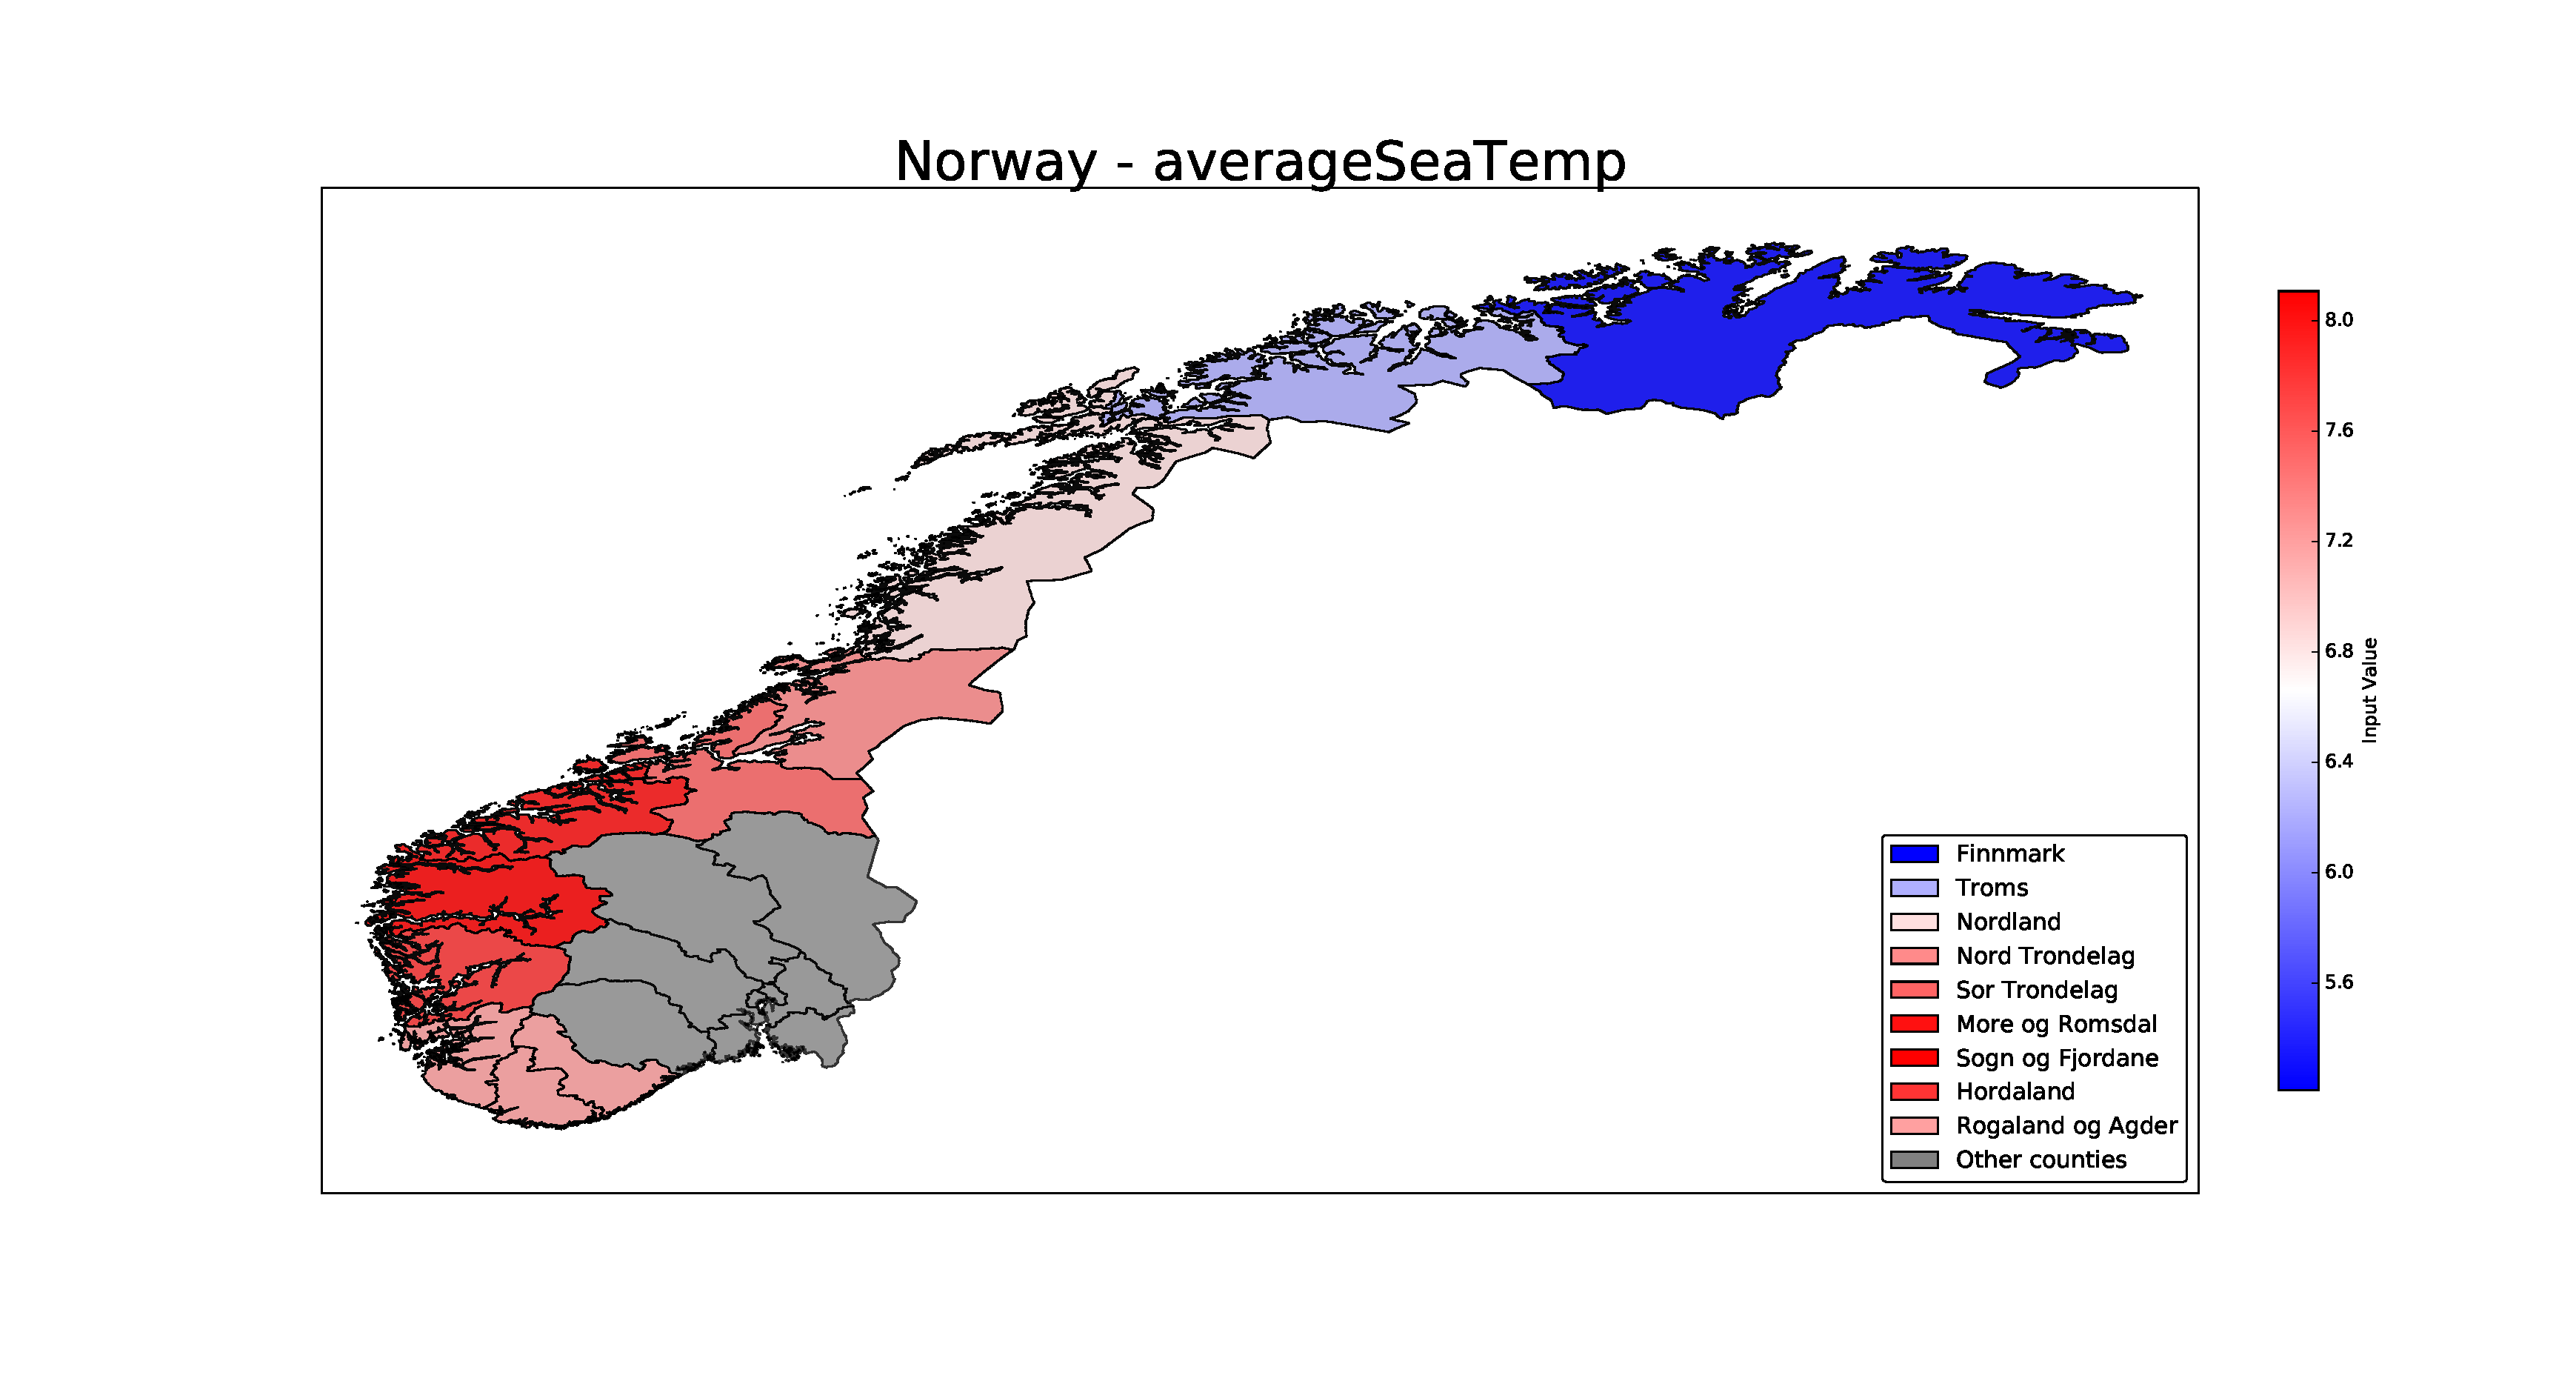
\includegraphics[trim={0 4cm 0 3cm},clip,width=1.3\textwidth]{Files/norway_averageSeaTemp.pdf}}
    \caption{Monthly average sea temperature from 2007 to 2014 in Norway}
    \label{fig: Norway_averageSeaTemp}
\end{figure}

\begin{figure}[H]
	\makebox[\textwidth][c]{
    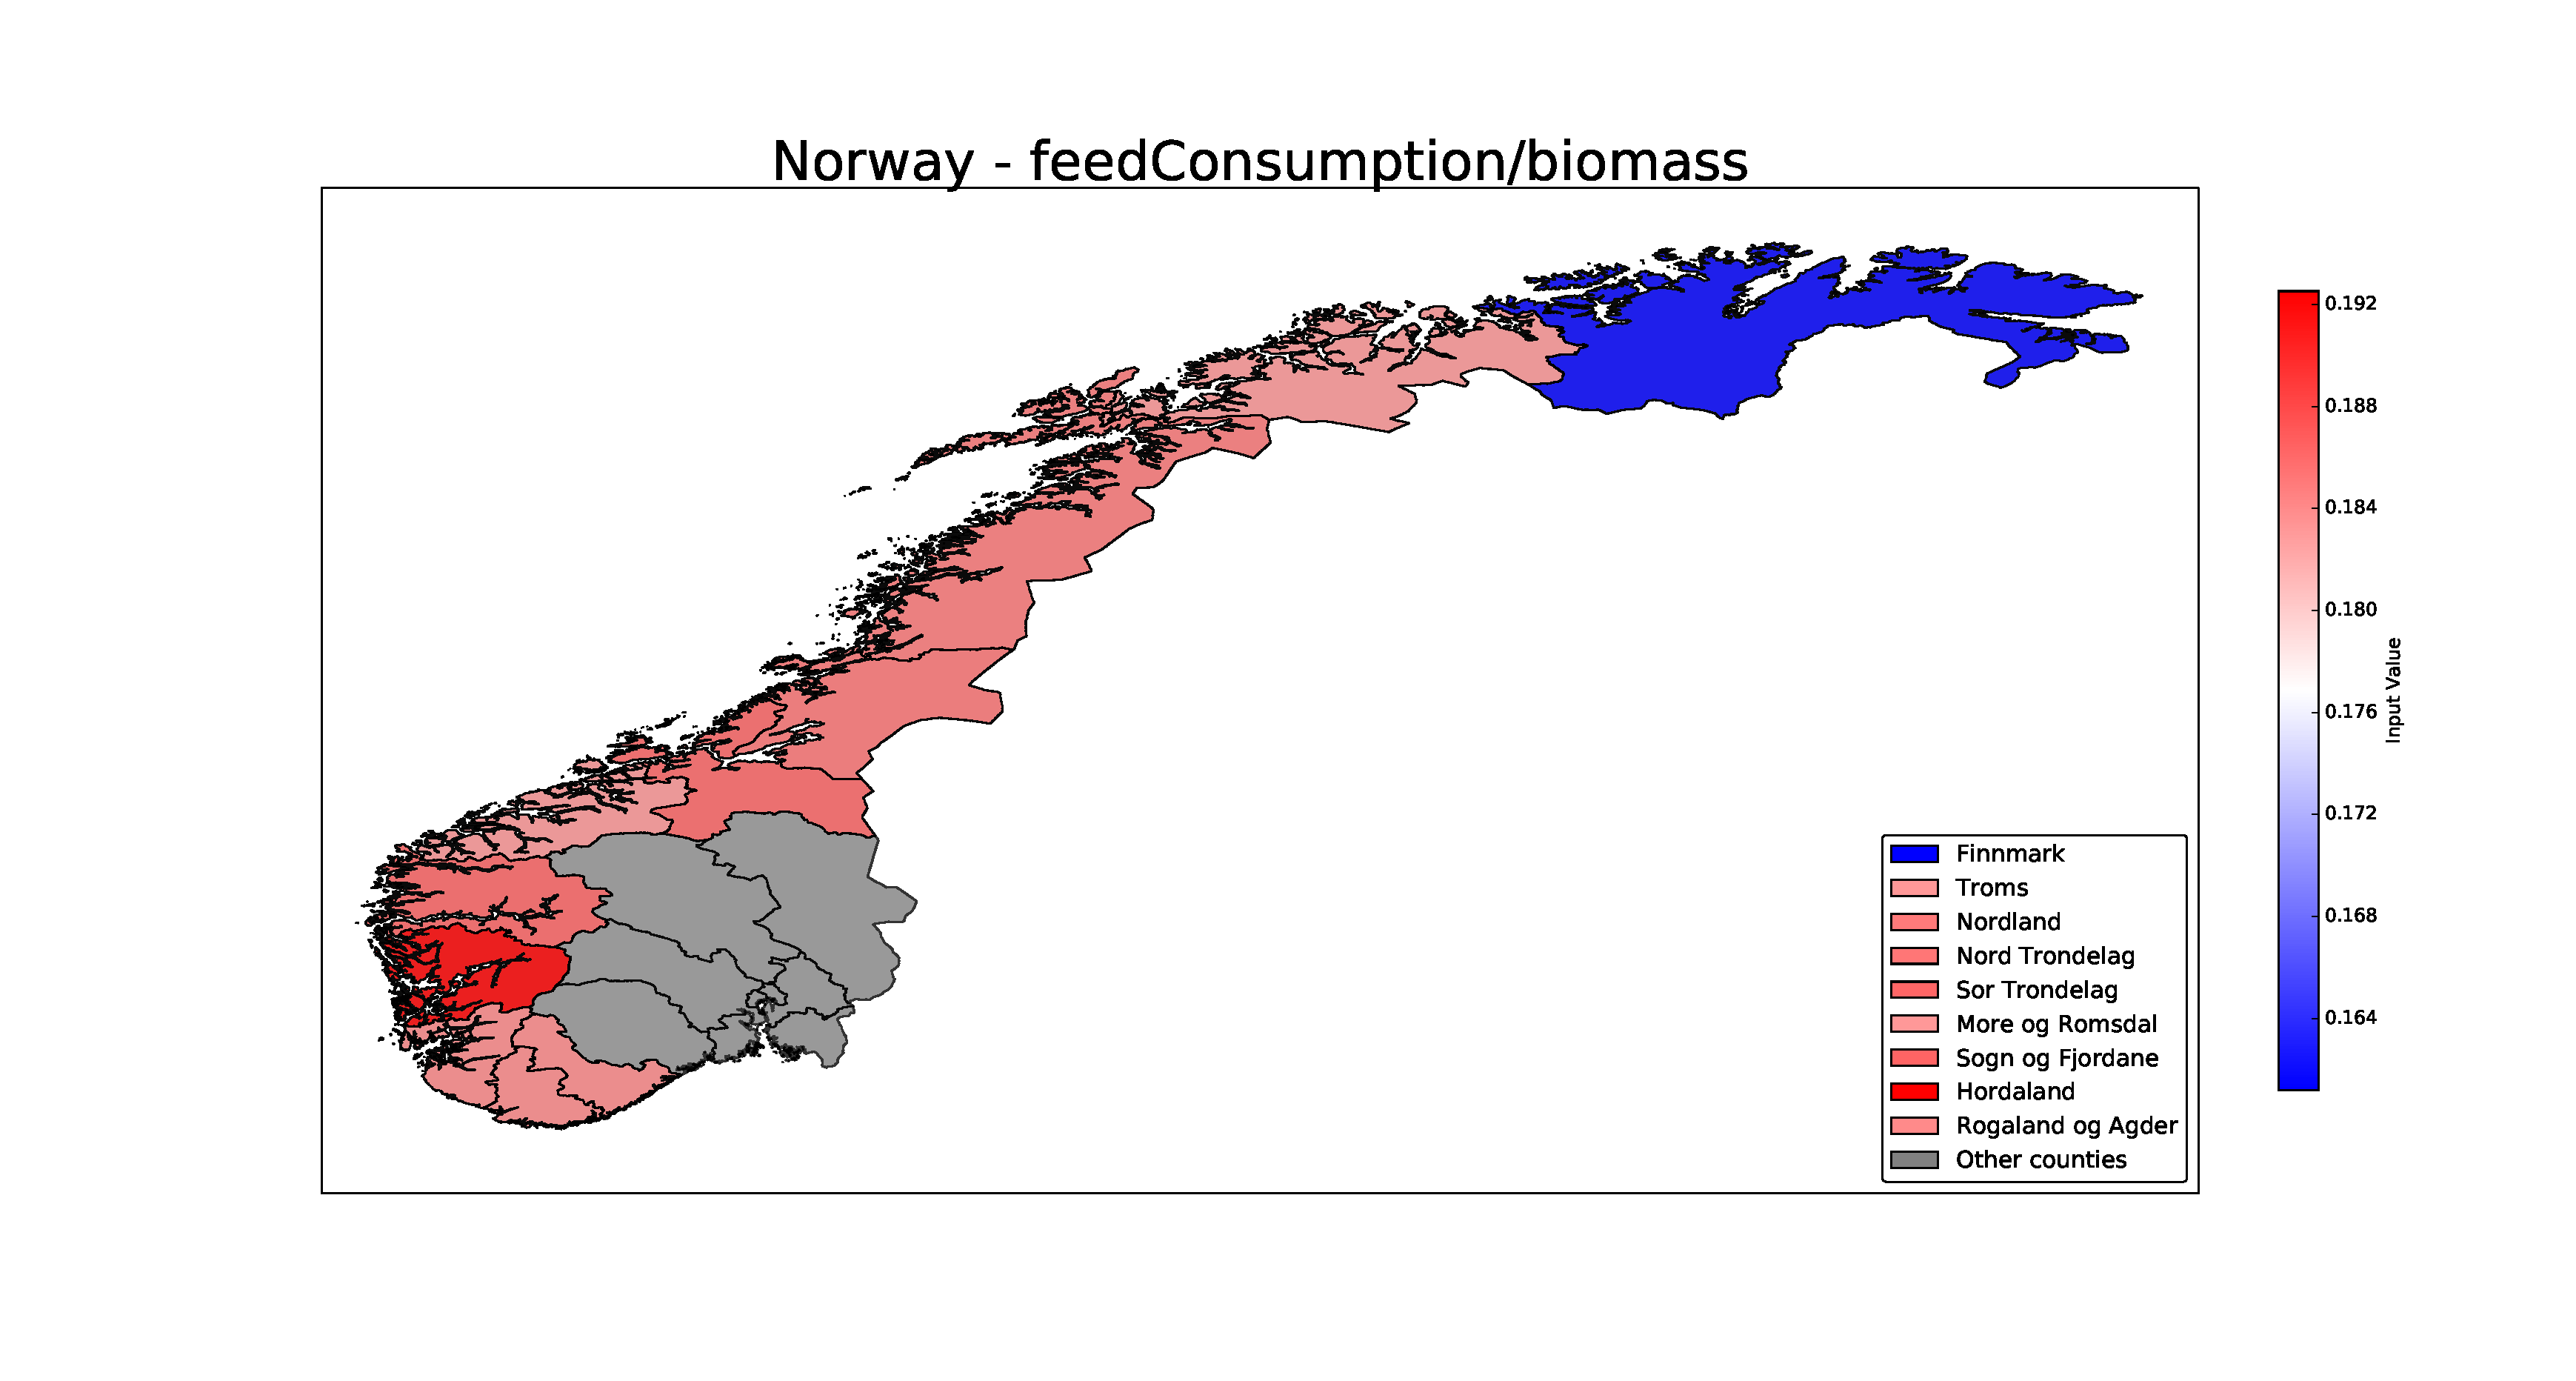
\includegraphics[trim={0 4cm 0 3cm},clip,width=1.3\textwidth]{Files/norway_feed-biomass.pdf}}
    \caption{Monthly average feed consumption per biomass from 2007 to 2014 in Norway}
    \label{fig: Norway_feed-biomass}
\end{figure}

\newpage

Further more, how is possible to check below here, also the correlation coefficient values calculated between all the parameter confirm what reported above.\\
\makebox[1\textwidth][c]{
\begin{minipage}[t]{0.6\textwidth}
\begin{figure}[H]
    \includegraphics[trim={0 0 0 0},clip,width=1\textwidth]{Files/Finnmark_Total_Matrix.pdf}
    \caption{Correlation matrix between all the parameters of the dataset about Finnmark}
    \label{fig: Finnmark_parametersComparison}
\end{figure}
\end{minipage} \hfill
\begin{minipage}[t]{0.6\textwidth}
\begin{figure}[H]
	\centering
    \includegraphics[trim={0 0 0 0},clip,width=1\textwidth]{Files/Troms_Total_Matrix.pdf}
    \caption{Correlation matrix between all the parameters of the dataset about Troms}
    \label{fig: Troms_parametersComparison}
\end{figure}
\end{minipage}}
\makebox[1\textwidth][c]{
\begin{minipage}[t]{0.6\textwidth}
\begin{figure}[H]
    \includegraphics[trim={0 0 0 0},clip,width=1\textwidth]{Files/Nordland_Total_Matrix.pdf}
    \caption{Correlation matrix between all the parameters of the dataset about Nordland}
    \label{fig: Nordland_parametersComparison}
\end{figure}
\end{minipage} \hfill
\begin{minipage}[t]{0.6\textwidth}
\begin{figure}[H]
	\centering
    \includegraphics[trim={0 0 0 0},clip,width=1\textwidth]{Files/Hordaland_Total_Matrix.pdf}
    \caption{Correlation matrix between all the parameters of the dataset about Hordaland}
    \label{fig: Hordaland_parametersComparison}
\end{figure}
\end{minipage}}

\vspace{+10mm}

I decided to focus on this particular parameter because, also if it's already known that is possible to feed the salmon more when the temperature is higher, it could be very useful for an implementation of a future prediction system.\\
It means that, during the forecasting of future feed consumption values, the sea average temperature would be considered for improve the final results.

\newpage

\section{Evaluation and limitations of the study}
\vspace{-5mm}
This study has a number of possible limitations, mainly due to a lack of background knowledge and experience about the current area, and also because of the relatively short time available.

ABOUT PYTHON RESULTS:
\vspace{-5mm}
\begin{itemize}
 \setlength{\itemsep}{-5pt}
\item PRO: The implemented Python system has a quite high reusability. It means that is possible to use it also with dataset filled with data parameter coming from other area of interest.
\item CONS: The implemented system in this thesis is probably efficient and productive for a personal use. That's because there is no GUI implemented and to change the customization of the output graphics you have to know Python language.
\item CONS: Not enough informations about machine learning field, so during this thesis was implemented just a basic implementation of the forecasting system, just to give an idea about how it works and give the possibility to improve it in future works.
\end{itemize}


ABOUT DATA ANALYSIS RESULTS:
\vspace{-5mm}
\begin{itemize}
 \setlength{\itemsep}{-5pt}
 \item PRO: Well structured datasets provided
 \item PRO: Usability of the results 
 \item CONS: Since the data sources are public, it's not possible to know the real reliability of it.
 \item CONS: The data collected are allowing just limitated analysis.
 \item CONS: Not enough informations have been extracted from the data cause of a lack in the background theory about Norwegian salmon farming, and not enough time to document myself in a proper way.
\end{itemize}


